Certificador: componente de PPA que "certifica" las demostraciones,
    generando un certificado en deducción natural. Implicó escribir muchos
    meta-teoremas.
    \begin{itemize}
        \item Formalización de muchos teoremas y axiomas: contextos (vale en el prefijo)
        \item Proof y proof steps, simplificación de la interfaz y mapeo de
        comandos a steps
        \item Implementación de cada comando
        \item By y solver para resolver varios. DNF. Extensión con foralls
        consecutivos. Demostración / justificación de que es correcto y completo
        para LP, pero heurístico para LPO (mostrar un caso en el que no funcione)
        \item Descarga de conjunciones
        \item Uso de dneg elim como razonamiento por el absurdo para demostrar
        deMorgan y equivalencias.
    \end{itemize}

En la sección pasada vimos cómo se puede usar PPA para demostrar teoremas. Pero,
¿cómo funciona por detrás? ¿Como asegura la validez lógica de las
demostraciones escritas por el usuario?

\section{Certificados}

Los programas de PPA se \textbf{certifican}, generando una demostración en
deducción natural. ¿Por qué? El lenguaje de PPA es complejo, la implementación
no es trivial. Si se escribe una demostración, para confiar en que es correcta
hay que confiar en la implementación de PPA.

Pero si PPA genera una demostración de bajo nivel, que usa las reglas de un
sistema lógico simple como deducción natural, entonces cualquiera que desconfíe
podría fácilmente escribir un chequeador, o usar uno confiable. Por eso genera
demostraciones en deducción natural, haciendo que cumpla con el \textbf{criterio
de de Bruijn}

\begin{definition}[Criterio de de Bruijn \cite{freek-bruijn}] Un asistente de
    demostración que satisface que sus demostraciones puedan ser chequeadas por
    un programa independiente, pequeño y confiable se dice que cumple con el
    criterio de de Bruijn.
\end{definition}

El módulo de PPA que \textit{certifica} las demostraciones de alto nivel de PPA
generando una demostración en deducción natural es el \modCertifier{}. Si
bien toda demostración que genere debería ser correcta, para atajar posibles
errores siempre se chequean con el \modChecker{} de DN.


\duda{Para pablo: pero si emite certificados que no corresponden a la demo original y chequean siempre, por ej. siempre el mismo, no estaría mal igual? Tenés que confiar también en la parte que emite el certificado.}

\section{Certificador}

El \modCertifier{} en realidad no genera una sola demostración de deducción
natural, sino que al poder haber más de un teorema en un archivo PPA, este
genera un \textbf{contexto} compuesto por una lista ordenada de
\textbf{hipótesis}. Hay dos tipos

\begin{itemize}
    \item Teoremas: Son fórmulas con demostraciones asociadas.
    \item Axiomas: Son fórmulas que se asumen válidas (pueden ser usadas para
    modelar una teoría)
\end{itemize}

\begin{figure}[H]
    \centering
    \begin{multicols}{2}
        \begin{tabular}{c}
            \lstinputlisting{listings/certifier/two-theorems.ppa}
        \end{tabular}
        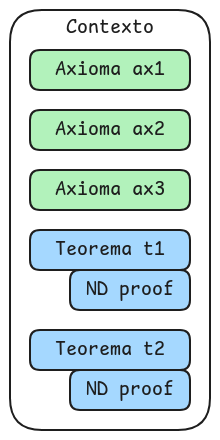
\includegraphics[scale=0.5]{img/ppa-context.png}
    \end{multicols}
    \caption{Contexto resultante de certificar de un programa}
\end{figure}


Por lo tanto, en vez de chequear demostraciones, se chequean contextos: Una
demostración será válida en el \textit{prefijo estricto del contexto} que la
contiene. Es decir, a la hora de chequearla, se deben asumir como ciertas todas
las hipótesis que fueron definidas previamente.

Pero no solo los axiomas y teoremas declarados en el programa se agregan al
contexto. Cada demostración de un teorema tendrá además un \textit{contexto
local} que extiende al anterior, solo en el marco de su demostración. Las
afirmaciones auxiliares que no afectan la tesis (\lstinline{have},
\lstinline{claim}, \lstinline{consider}, etc.) se agregan como teoremas. Por lo
tanto, cuando se citen, se pegan sus demostraciones. Por otro lado, algunos
comandos agregan axiomas, los mismos que en deducción natural agregan fórmulas
al contexto (\lstinline{suppose} y \lstinline{consider}). Es correcto asumir
como ciertas esas hipótesis, porque lo mismo se hará durante el chequeo de la
demostración en deducción natural.

\begin{figure}[H]
    \centering
    \begin{multicols}{2}
        \begin{tabular}{c}
            \lstinputlisting{listings/certifier/local-context.ppa}
        \end{tabular}
        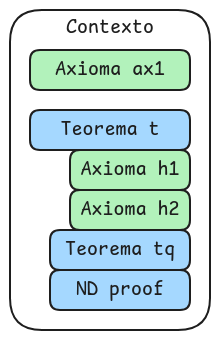
\includegraphics[scale=0.5]{img/ppa-local-context.png}
    \end{multicols}
    \caption{Contexto local}
\end{figure}

\section{Funcionamiento del by}

El \lstinline{by} es el mecanismo principal de demostración en PPA, y el corazón del \modCertifier. Genera
\textbf{automáticamente} una demostración de que una fórmula es consecuencia lógica de
una lista de hipótesis.

Sea $A$ una fórmula. Supongamos que queremos demostrar \lstinline{thus A by h1, ..., hn} y que en el contexto tenemos que las hipótesis $h_i$ corresponden a
fórmulas $\formTwo_i$, con $i \in \{1, ..., n\}, n \in \setNaturals$. Primero
veamos la idea general de la estrategia y luego profundizamos en cada paso.

Los pasos para certificar un \lstinline{by} son,

\begin{itemize}
    \item Queremos demostrar la implicación de las hipótesis a la fórmula. La
    llamamos \textbf{tesis}.
    \[
        \formTwo_1 \fAnd \dots \fAnd \formTwo_n \fImp \form
    \]
    \item Razonamos por el absurdo: asumiendo la negación de la tesis encontramos una contradicción
    \begin{align*}
        \fNot (\formTwo_1 \fAnd \dots \fAnd \formTwo_n \fImp \form)
        &\equiv \fNot (\fNot (\formTwo_1 \fAnd \dots \fAnd \formTwo_n) \fOr \form)\\
        &\equiv \formTwo_1 \fAnd \dots \fAnd \formTwo_n \fAnd \fNot \form
    \end{align*}
    \item Convertimos la negación de la tesis a forma normal disyuntiva (DNF),
    una disyunción de conjunciones de literales (``cláusulas'').
    \[
        (\formLit^1_{1} \fAnd \dots \fAnd \formLit^1_{n_1})
        \fOr \dots \fOr
        (\formLit^m_{1} \fAnd \dots \fAnd \formLit^m_{n_m})
    \]

    donde $m \in \setNaturals$ es el número de cláusulas, $n_1, \dots, n_m \in
    \setNaturals$ es la cantidad de fórmulas de cada cláusula y $\formLit^i_j$
    es la $j$-ésima fórmula de la $i$-ésima cláusula.
    \item Buscamos una contradicción refutando cada cláusula individualmente.
    Una cláusula $\formLit_1 \fAnd \dots \fAnd \formLit_n$ será refutable si
    cumple una de las siguientes condiciones.
    \begin{itemize}
        \item Contiene $\fFalse$
        \item Contiene dos fórmulas opuestas ($\formLit, \fNot \formLit$)
        \item Eliminando existenciales consecutivos y re-convirtiendo a DNF, se
        consigue una refutación ($\fNot \pred(k), \forall \var .\ \pred(x)$)
    \end{itemize}
\end{itemize}

La complejidad del mecanismo no reside solo en tener que realizar todos estos
pasos, sino que el desafío principal fue \textbf{generar la demostración en
deducción natural}. Veamos un ejemplo sin generar la demostración, sin
eliminación de existenciales.

\begin{ejemplo}[Ejemplo sin cuantificadores]
    Tenemos el siguiente programa

    \begin{figure}[H]
        \centering
        \begin{tabular}{c}
            \lstinputlisting{listings/certifier/by-modus-ponens.ppa}
        \end{tabular}
    \end{figure}

    Para certificar \lstinline{thus b by ax1, ax2} hay que generar una
    demostración para la implicación $\big((a \fImp b) \wedge a \big)\fImp b$.

    \begin{enumerate}
        \item Negamos la fórmula 
        \[ \fNot [ \big( (a \to b) \fAnd a \big) \to b ] \]

        \item La convertimos a DNF
        \todo{Cambiar x e y}
        \begin{align*}
            &\fNot [ \big( (a \to b) \fAnd a \big) \to b ] \\
            &\equiv \fNot [ \fNot \big( (a \to b) \fAnd a \big) \fOr b ]
                && (x \to y \equiv \fNot x \fOr y)\\
            &\equiv \fNot \fNot \big( (a \to b) \fAnd a \big) \fAnd \fNot b
                && (\fNot(x \fOr y) \equiv \fNot x \fAnd \fNot y)\\
            &\equiv \big( (a \to b) \fAnd a \big) \fAnd \fNot b
                && (\fNot\fNot x \equiv x)\\
            &\equiv (\fNot a \fOr b) \fAnd a \fAnd \fNot b
                 && (x \to y \equiv \fNot x \fOr y)\\
            &\equiv (\fNot a \fOr b) \fAnd a \fAnd \fNot b
                && ((x \fOr y) \fAnd z \equiv (x \fAnd z) \fOr (y \fAnd z))\\
            &\equiv
                (\fNot a \fAnd a \fAnd \fNot b)
                \vee
                (b \fAnd a \fAnd \fNot b)
        \end{align*}

        \item Buscamos una contradicción refutando cada cláusula
        \begin{itemize}
            \item $(\fNot a \fAnd a \fAnd \fNot b)$ tenemos $\fNot a$ y $a$.
            \item $(b \fAnd a \fAnd \fNot b)$ tenemos $b$ y $\fNot b$.
        \end{itemize}
    \end{enumerate}
\end{ejemplo}


\subsection{Razonamiento por el absurdo}
\label{ppa-cert:sec:abs-reasoning}

Queremos asumir que no vale la fórmula original, es decir $\fNot (\formTwo_1
\fAnd \dots \fAnd \formTwo_n \fImp \form)$, y llegar a una contradicción. Pero
en la demostración que estamos generando de deducción natural, tenemos que
demostrar $(\formTwo_1 \fAnd \dots \fAnd \formTwo_n \fImp \form)$. ¿Cómo se
puede razonar por el absurdo?

De la misma forma que en la \namedref{nd:sec:admissible-rules} se introduce
\textit{modus tollens} como una regla admisible, para razonar por el absurdo
vamos a usar la \textbf{eliminación de la doble negación}. Es un principio de
razonamiento clásico que es equivalente a LEM.


\begin{theorem}[Eliminación de la doble negación]
    Sea $\form$ una fórmula cualquiera. Vale $\fNot \fNot \form \judG \form$, y lo notamos como regla admisible

    \begin{prooftree}
        \AxiomC{}
        \RL{\ruleDnegE}
        \admissibleRuleLine
        \UnaryInfC{$\fNot \fNot \form \judG \form$}
    \end{prooftree}
\end{theorem}
\begin{proof}
    En deducción natural,

    \begin{prooftree}
        \def\defaultHypSeparation{\hskip .1in} % default .2in
        \AxiomC{}
        \LL{\ruleLEM}
        \UnaryInfC{$\fNot \fNot \form \judG \form \fOr \fNot \form$}
        \AxiomC{}
        \RL{\ruleAx}
        \UnaryInfC{\(
            \fNot \fNot \form, \form \judG \form
        \)}
        \AxiomC{}
        \LL{\ruleAx}
        \UnaryInfC{\(
            \fNot \fNot \form, \fNot\form \judG \fNot \fNot \form
        \)}
        \AxiomC{}
        \RL{\ruleAx}
        \UnaryInfC{\(
            \fNot \fNot \form, \fNot\form \judG \fNot \form
        \)}
        \RL{\ruleNotE}
        \BinaryInfC{\(
            \fNot \fNot \form, \fNot \form \judG \form
        \)}
        \RL{\ruleOrE}
        \TrinaryInfC{$\fNot \fNot \form \judG \form$}
    \end{prooftree}
\end{proof}

¿Cómo lo usamos? Introducimos otra regla admisible: \textbf{cut}, que nos
permite ``pegar'' demostraciones entre sí. Si estamos queriendo demostrar
$\form$, y queremos reducir el problema a $\formTwo$ que sí podemos probar, esta
regla nos permite hacerlo.

\begin{theorem}[Cut] La siguiente regla de inferencia es admisible
\begin{prooftree}
    \AxiomC{$\ctx, \formTwo \judG \form$}
    \AxiomC{$\ctx \judG \formTwo$}
    \RL{\ruleCut}
    \admissibleRuleLine
    \BinaryInfC{$\ctx \judG \form$}
\end{prooftree}
\end{theorem}

\begin{proof}
    La regla \ruleCut{} se puede ver como un \textit{macro} que por atrás genera
    la siguiente demostración
    
    \begin{prooftree}
        \AxiomC{$\ctx, \formTwo \judG \form$}
        \RL{\ruleImpI}
        \UnaryInfC{$\ctx \judG \formTwo \fImp \form$}
        \AxiomC{$\ctx \judG \formTwo$}
        \RL{\ruleImpE}
        \BinaryInfC{$\ctx \judG \form$}
    \end{prooftree}
\end{proof}

\begin{ejemplo}
Cut nos permite continuar la demostración por otra fórmula a partir de la cual
podamos demostrar la original. Sean $\someProof_{\formTwo \fImp \form}$ una
demostración de $\formTwo \judG \form$ y $\someProof_\formTwo$ una demostración
de $\formTwo$ (la continuación). Podemos usar cut de la siguiente manera.

\begin{prooftree}
    \AxiomC{$\someProof_{\formTwo \fImp \form}$}
    \noLine
    \UnaryInfC{$\ctx, \formTwo \judG \form$}
    \AxiomC{$\someProof_\formTwo$}
    \noLine
    \UnaryInfC{$\ctx \judG \formTwo$}
    \RL{\ruleCut}
    \admissibleRuleLine
    \BinaryInfC{$\ctx \judG \form$}
\end{prooftree}

Que es generado como

\begin{prooftree}
    \AxiomC{$\someProof_{\formTwo \fImp \form}$}
    \noLine
    \UnaryInfC{$\ctx, \formTwo \judG \form$}
    \RL{\ruleImpI}
    \UnaryInfC{$\ctx \judG \formTwo \fImp \form$}
    \AxiomC{$\someProof_\formTwo$}
    \noLine
    \UnaryInfC{$\ctx \judG \formTwo$}
    \RL{\ruleImpE}
    \BinaryInfC{$\ctx \judG \form$}
\end{prooftree}
\end{ejemplo}

\begin{lemma}[Razonamiento por el absurdo] Imaginemos que queremos demostrar
$\form$ por el absurdo. Podemos juntar con cut con la eliminación de la doble
negación, pasando a demostrar $\fNot \fNot \form$, que para introducirla,
debemos demostrar $\ctx, \fNot \form \judG \fFalse$. Es decir, asumiendo que no
es cierta la fórmula, deducimos una contradicción. Justo lo que estábamos
buscando para razonar por el absurdo.

\begin{prooftree}
    \AxiomC{}
    \RL{\ruleDnegE}
    \admissibleRuleLine
    \UnaryInfC{$\ctx, \fNot \fNot \form \judG \form$}
    \AxiomC{$\vdots$}
    \noLine
    \UnaryInfC{$\ctx, \fNot \form \judG \fFalse$}
    \RL{\ruleNotI}
    \UnaryInfC{$\ctx \judG \fNot\fNot \form$}
    \RL{\ruleCut}
    \admissibleRuleLine
    \BinaryInfC{$\ctx \judG \form$}
\end{prooftree}
\end{lemma}

\begin{obs}
    A \ruleDnegE{} La formulamos como $\fNot \fNot \form \judG \form$ y la usamos con
    \textbf{cut}, pero otra alternativa equivalente, levemente más tediosa para
    generar demostraciones, hubiera sido demostrarla como $\fNot \fNot \form
    \fImp \form$ y usarla con \ruleImpE{} directamente.
\end{obs}

\subsection{DNF}

Tenemos que generar una demostración de que la negación de la tesis genera una
contradicción, pero lo queremos hacer a partir de la tesis en DNF.

\begin{definition}[DNF]
    Una fórmula está en \textbf{forma normal disyuntiva} o DNF
    (\textit{disjunctive normal form}) si es una disyunción de conjunciones de
    literales.  Llamamos \textbf{cláusulas} a las conjunciones que la
    componen. Un literal será un predicado, una negación de un predicado o una
    fórmula cualquiera que comienza con un cuantificador. Ejemplos:
    
    \begin{itemize}
        \item $\formLit \fAnd \formLitTwo$ está en DNF
        \item $(\formLit \fAnd \formLitThree) \fOr (\formLit \fAnd \formLitTwo)$ también
        \item $(\formLit \fImp \formLitTwo) \fOr (\formLit \fAnd \formLitTwo)$ no lo está
        \item $\big(\forall \var . (\formLit \fImp \formLitTwo)\big) \fOr (\formLit \fAnd \formLitTwo)$ si.
    \end{itemize}
\end{definition}

\begin{theorem}[Conversión a DNF] Para toda fórmula $\form$, existe
    $\dnf{\form}$ su equivalente en DNF. Y vale $\form \judG \dnf{\form}$.
\end{theorem}

\begin{obs}
    Continuamos la demostración por la refutación de la fórmula en DNF mediante
el uso de cut.

\begin{prooftree}
    \AxiomC{\vdots}
    \noLine
    \UnaryInfC{$\ctx, \form \judG \dnf{\form}$}
    \AxiomC{\vdots}
    \noLine
    \UnaryInfC{$\ctx, \form, \dnf{\form} \judG \fFalse$}
    \RL{\ruleCut}
    \admissibleRuleLine
    \BinaryInfC{$\ctx, \form \judG \fFalse$}
\end{prooftree}
\end{obs}


Para convertir una fórmula cualquiera a DNF, vamos a implementar una traducción
\textit{small-step} implementando el siguiente sistema de reescritura.

\begin{figure}[H]
    \begin{align*}
        \fNot\fNot \formLit &\rightsquigarrow
            \formLit
            &&\text{eliminación de $\fNot\fNot$}\\
        \fNot \fFalse &\rightsquigarrow
            \fTrue\\
        \fNot \fTrue &\rightsquigarrow
            \fFalse\\
        \formLit \fImp \formLitTwo &\rightsquigarrow
            \fNot \formLit \fOr \formLitTwo
            &&\text{definición de implicación}\\
        \fNot(\formLit \fOr \formLitTwo) &\rightsquigarrow
            \fNot \formLit \fAnd \fNot \formLitTwo
            &&\text{distributiva de $\fNot$ sobre $\fAnd$}\\
        \fNot(\formLit \fAnd \formLitTwo) &\rightsquigarrow
            \fNot \formLit \fOr \fNot \formLitTwo
            &&\text{distributiva de $\fNot$ sobre $\fOr$}\\
        (\formLit \fOr \formLitTwo) \fAnd \formLitThree &\rightsquigarrow
            (\formLit \fAnd \formLitThree) \fOr (\formLitTwo \fAnd \formLitThree)
            &&\text{distributiva de $\fAnd$ sobre $\fOr$ (der)}\\
        \formLitThree \fAnd (\formLit \fOr \formLitTwo) &\rightsquigarrow
            (\formLitThree \fAnd \formLit) \fOr (\formLitThree \fAnd \formLitTwo)
            &&\text{distributiva de $\fAnd$ sobre $\fOr$ (izq)}\\
        \formLit \fOr (\formLitTwo \fOr \formLitThree) &\rightsquigarrow
            (\formLit \fOr \formLitTwo) \fOr \formLitThree
            &&\text{asociatividad de $\fOr$}\\
        \formLit \fAnd (\formLitTwo \fAnd \formLitThree) &\rightsquigarrow
            (\formLit \fAnd \formLitTwo) \fAnd \formLitThree
            &&\text{asociatividad de $\fAnd$}
    \end{align*}    
    \caption{Sistema de reescritura para conversión a DNF de forma sintáctica}
\end{figure}

Para su implementación, no podemos hacerlo meramente de forma sintáctica, sino
que tenemos \textit{generar una demostración} para cada equivalencia. Además,
hay casos en donde tenemos que reemplazar una sub-fórmula por una equivalente.
En ese caso usamos la \textit{congruencia} de los operadores, que también
tuvimos que demostrar. Por ejemplo en
\[
    \formLit \fOr \bm{\fNot (\formLitTwo \fOr \formLitThree)}
    \equiv
    \formLit \fOr \bm{(\fNot \formLitTwo \fAnd \fNot \formLitThree)}
\]
donde reescribimos $\fNot
(\formLitTwo \fOr
\formLitThree) \equiv (\fNot \formLitTwo \fAnd \fNot \formLitThree)$ manteniendo el
resto.

\begin{figure}[H]
    \begin{align*}
        \form \judG \form'
            &\Rightarrow \form \fAnd \formTwo \judG \form' \fAnd \formTwo\\
        \form \judG \form'
            &\Rightarrow \form \fOr \formTwo \judG \form' \fOr \formTwo\\
        \form' \judG \form
            &\Rightarrow \fNot \form \judG \fNot \form'
    \end{align*}
    \caption{Congruencias}
\end{figure}

No hay regla de congruencia para $\fImp$ pues se convierte en un $\fOr$. Es
sumamente importante observar que $\fNot$ es \textit{contravariante}, para
demostrar $\fNot \form \judG \fNot \form'$ no necesitamos tener una demostración
de $\form \judG \form'$, sino de $\form' \judG \form$. Esto quiere decir que
para todas las equivalencias, incluso las congruencias, no nos alcanza con
demostrarlas en un solo sentido (por ej. $\fNot(\formLit \fOr \formLitTwo) \judG
\fNot \formLit \fAnd \fNot \formLitTwo$) sino que vamos a necesitar ambos, la
ida y la vuelta:
\(
    \fNot(\formLit \fOr \formLitTwo)
        \judG \fNot \formLit \fAnd \fNot \formLitTwo
\) y \(
    \fNot \formLit \fAnd \fNot \formLitTwo \judG \fNot(\formLit \fOr \formLitTwo)
\). lo notamos como \[
    \fNot(\formLit \fOr \formLitTwo)
        \judgEquiv \fNot \formLit \fAnd \fNot \formLitTwo
\]

\subsubsection{Algoritmo}

Finalmente, el algoritmo para generar la demostración de la conversión de una
fórmula en DNF se implementa de forma \textit{small-step}. Es la clausura de
hacer un ``paso'' de la conversión a DNF, que puede o bien ser un paso de
reescritura, o uno de congruencia reescribiendo una sub-fórmula. En cada uno se
usa una de las siguientes demostraciones.

\begin{figure}[H]
    \begin{align*}
        \intertext{Pasos base}
        \fNot\fNot \formLit &\judgEquiv
            \formLit
            \\
        \fNot \fFalse &\judgEquiv
            \fTrue\\
        \fNot \fTrue &\judgEquiv
            \fFalse\\
        \formLit \fImp \formLitTwo &\judgEquiv
            \fNot \formLit \fOr \formLitTwo
            \\
        \fNot(\formLit \fOr \formLitTwo) &\judgEquiv
            \fNot \formLit \fAnd \fNot \formLitTwo
            \\
        \fNot(\formLit \fAnd \formLitTwo) &\judgEquiv
            \fNot \formLit \fOr \fNot \formLitTwo
            \\
        (\formLit \fOr \formLitTwo) \fAnd \formLitThree &\judgEquiv
            (\formLit \fAnd \formLitThree) \fOr (\formLitTwo \fAnd \formLitThree)
            \\
        \formLitThree \fAnd (\formLit \fOr \formLitTwo) &\judgEquiv
            (\formLitThree \fAnd \formLit) \fOr (\formLitThree \fAnd \formLitTwo)
            \\
        \formLit \fOr (\formLitTwo \fOr \formLitThree) &\judgEquiv
            (\formLit \fOr \formLitTwo) \fOr \formLitThree
            \\
        \formLit \fAnd (\formLitTwo \fAnd \formLitThree) &\judgEquiv
            (\formLit \fAnd \formLitTwo) \fAnd \formLitThree\\
        \intertext{Pasos recursivos de congruencia (con $\form \judgEquiv \form'$)}
        \form \fAnd \formTwo &\judgEquiv \form' \fAnd \formTwo\\
        \form \fOr \formTwo &\judgEquiv \form' \fOr \formTwo\\
        \fNot \form &\judgEquiv \fNot \form'
    \end{align*}
    \caption{Pasos de conversión a DNF}
\end{figure}


En total son 26 demostraciones. Nos ahorramos los detalles porque son bien
conocidas (por ej. DeMorgan).

\duda{Demostración de que termina? De que es correcto? Al menos una cita para que sea más confiable el sistema de reescritura? O se asume como bien conocido?}

\subsection{Contradicciones}

Tenemos la fórmula traducida a DNF. Debemos demostrar una contradicción a partir
de ella. Si tenemos las cláusulas $\clause_1 \fOr \clause_2$, podemos demostrar
$\clause_1 \fOr \clause_2 \judG \fFalse$ usando \ruleOrE{} y a partir de cada
una, llegando a una contradicción. Esto se generaliza a N cláusulas mediante el
uso \ruleOrE{} anidados. Por esto decimos que hay que \textit{``refutar cada
cláusula''}. El método tiene tres formas de refutarlas

\begin{itemize}
    \item Contienen fórmulas opuestas: $\form \fAnd \fNot \form$ (con
    \ruleNotE{})
    \item Contienen $\fFalse$
    \item Eliminando cuantificadores universales consecutivos (próxima sección)
\end{itemize}

Para los primeros dos, es necesario demostrar a partir de la cláusula una
fórmula. Pero como pueden tener una cantidad arbitraria, según cómo esté
asociado el $\fAnd$, una demostración a mano de
\(
    \form_1 \fAnd \dots \fAnd \form_i \fAnd \dots \fAnd \form_n \judG \form_i,
\)
puede ser muy engorrosa. Como las reglas son binarias, hay que
usar \ruleAndEOne{} y \ruleAndETwo{} anidados. Para simplificarlo demostramos
otra regla admisible, la proyección de un elemento \ruleAndEProj{\anyForm}.

\begin{theorem}[Regla admisible \ruleAndEProj{\anyForm}]
    Sea $\anyForm$ alguna fórmula de la conjunción $\anyForm_1 \fAnd \dots \fAnd
    \anyForm_i$. Notamos por \ruleAndEProj{\anyForm} a la proyección \textit{de
    la fórmula}, sin importar en qué posición de la conjunción está.

    \begin{prooftree}
        \AxiomC{$\ctx \judG \anyForm_1 \fAnd \dots \fAnd \anyForm_i \fAnd \dots \fAnd \anyForm_n$}
        \AxiomC{$n \in \setNaturals$}
        \admissibleRuleLine
        \RL{\ruleAndEProj{\anyForm_{i}}}
        \BinaryInfC{$\ctx \judG \anyForm_i$}
    \end{prooftree}
\end{theorem}
\begin{proof}
    Para generar la demostración correspondiente usando \ruleAndEOne{} y
    \ruleAndETwo{}, basta con identificar el camino hacia $\anyForm_i$, y luego
    caminar recursivamente el $\fAnd$ usando \ruleAndEOne{} si el camino
    continúa por la izquierda y \ruleAndETwo{} si sigue por la derecha.
\end{proof}

\begin{ejemplo}[Contradicción]
    Veamos un ejemplo de las primeras dos formas de refutar cláusulas. Los
    cuantificadores universales los veremos en la siguiente sección.
\begin{prooftree}
    \AxiomC{}
    \LL{\ruleAx}
    \UnaryInfC{\(
        \ctx \judG (\fNot a \fAnd a \fAnd \fNot b)\vee (b \fAnd a \fAnd \fFalse)
    \)}
    \AxiomC{$\someProof_L$}
    \noLine
    \UnaryInfC{\(
        \ctx, \fNot a \fAnd a \fAnd \fNot b \judG \fFalse
    \)}
    \AxiomC{}
    \RL{\ruleAx}
    \UnaryInfC{$\ctx_1 \judG b \fAnd a \fAnd \fFalse$}
    \RL{\ruleAndEProj{\fFalse}}
    \admissibleRuleLine
    \UnaryInfC{\(
        \ctx, b \fAnd a \fAnd \fFalse \judG \fFalse
    \)}
    \RL{\ruleOrE}
    \TrinaryInfC{\(
        \ctx = (\fNot a \fAnd a \fAnd \fNot b)
        \vee
        (b \fAnd a \fAnd \fFalse)
        \judG
        \fFalse
    \)}
\end{prooftree}

donde

\begin{prooftree}
    \AxiomC{}
    \RL{\ruleAx}
    \UnaryInfC{$\ctx_1 \judG \fNot a \fAnd a \fAnd \fNot b$}
    \RL{\ruleAndEProj{\fNot a}}
    \admissibleRuleLine
    \UnaryInfC{$\ctx_1 \judG \fNot a$}
    \AxiomC{}
    \RL{\ruleAx}
    \UnaryInfC{$\ctx_1 \judG \fNot a \fAnd a \fAnd \fNot b$}
    \RL{\ruleAndEProj{a}}
    \admissibleRuleLine
    \UnaryInfC{$\ctx_1 \judG a$}
    \RL{\ruleNotE}
    \LL{$\someProof_L=$}
    \BinaryInfC{\(
        \ctx_1 = \ctx, b \fAnd a \fAnd \fFalse \judG \fFalse
    \)}
\end{prooftree}
\end{ejemplo}

\duda{No se si me convence la notación \ruleAndEProj{\alpha}, después de todo es
una proyección y se suele notar con $\Pi$, pero ese símbolo lo estamos usando
para representar demostraciones (ej. $\someProof_L$).}

\subsection{Eliminación de cuantificadores universales}

Hasta ahora logramos razonar por el absurdo, convertir la fórmula a DNF, y
encontrar una contradicción siempre que no haya que eliminar cuantificadores
universales. Pero es usual que en una teoría de primer orden, los axiomas
contengan cuantificadores universales y sea necesario eliminarlos para poder
demostrar un \lstinline{by}. Veamos un ejemplo.

\begin{ejemplo}[Ejemplo con cuantificadores]
    Tenemos el siguiente programa

    \begin{figure}[H]
        \centering
        \begin{tabular}{c}
            \lstinputlisting{listings/certifier/by-modus-ponens-quant.ppa}
        \end{tabular}
    \end{figure}

    Para certificar \lstinline{thus q(a) by ax1, ax2} hay que generar una
    demostración para la implicación \(
        \bigg(\Big(\forall x. (p(x) \fImp q(x))\Big) \wedge p(a) \bigg)
        \fImp q(a)
    \).

    \begin{enumerate}
        \item Negamos la fórmula 
        \[
            \fNot \left[
            \bigg(\Big(\forall x. (p(x) \fImp q(x))\Big) \wedge p(a) \bigg)
            \fImp q(a)
        \right]
        \]

        \item La convertimos a DNF
        \begin{align*}
            &\fNot [ \big( (a \to b) \fAnd a \big) \to b ] \\
            &\equiv \fNot [ \fNot \big( (a \to b) \fAnd a \big) \fOr b ]
                && (x \to y \equiv \fNot x \fOr y)\\
            &\equiv \fNot \fNot \big( (a \to b) \fAnd a \big) \fAnd \fNot b
                && (\fNot(x \fOr y) \equiv \fNot x \fAnd \fNot y)\\
            &\equiv \big( (a \to b) \fAnd a \big) \fAnd \fNot b
                && (\fNot\fNot x \equiv x)\\
            &\equiv (\fNot a \fOr b) \fAnd a \fAnd \fNot b
                 && (x \to y \equiv \fNot x \fOr y)\\
            &\equiv (\fNot a \fOr b) \fAnd a \fAnd \fNot b
                && ((x \fOr y) \fAnd z \equiv (x \fAnd z) \fOr (y \fAnd z))\\
            &\equiv
                (\fNot a \fAnd a \fAnd \fNot b)
                \vee
                (b \fAnd a \fAnd \fNot b)
        \end{align*}

        \item Buscamos una contradicción refutando cada cláusula
        \begin{itemize}
            \item $(\fNot a \fAnd a \fAnd \fNot b)$ tenemos $\fNot a$ y $a$.
            \item $(b \fAnd a \fAnd \fNot b)$ tenemos $b$ y $\fNot b$.
        \end{itemize}
    \end{enumerate}
\end{ejemplo}



\subsection{Unificación}
\label{ppa:sec:unification}

\subsection{Juntando demostraciones}

\todo{Cut como regla admisible}

\subsection{Poder expresivo}

\duda{Está bien decir poder expresivo?}

El solver implementado es \textbf{completo para lógica proposicional}, pero heurístico para lógica de primer orden. Esto es aceptable, puesto que la satisfacibilidad de lógica de primer orden es indecidible \todo{Cita?}, y además el objetivo del trabajo no fue dar el mejor solver, sino dar alguno.

\todo{Citar Hilbert 1950}
\begin{theorem}[El solver es completo para lógica proposicional]
    \todo{Demo}
\end{theorem}

\subsubsection{Limitaciones}

No puede demostrar por ej.

\todo{ejemplo elim 2 foralls}

\todo{otro ejemplo más burdamente complejo que requiera sat sovler}


\section{Comandos correspondientes a reglas de inferencia}

Como se puede apreciar en \fullref{ppa:tab:inference-rules-to-commands}, la
mayoría de los comandos se corresponden directamente con reglas de inferencia,
por lo que su traducción es más sencilla.

\todo{trad}

\section{Descarga de conjunciones}

\section{Comandos adicionales}

\todo{add}


